\documentclass{book}
\usepackage[english]{babel}     
\usepackage[utf8]{inputenc}     % accent symbols
\usepackage[T1]{fontenc}
\usepackage{lmodern}
\usepackage{microtype}
\usepackage{natbib}
\usepackage{tocbibind}          
\usepackage{amsmath}            % math symbols
\usepackage{amsthm}             % math symbols
\usepackage[colorlinks=true,linkcolor=red]{hyperref} % hyper link

% for code
\usepackage{listings}
\usepackage{color,xcolor}
\definecolor{mygreen}{rgb}{0,0.6,0}
\definecolor{mygray}{rgb}{0.9,0.9,0.9}
\definecolor{mymauve}{rgb}{0.58,0,0.82}
\lstset{
backgroundcolor=\color{mygray},
numbers=left,                    
columns=fullflexible,
breaklines=true,      
captionpos=b,         
tabsize=4,            
commentstyle=\color{mygreen}, 
escapeinside={\%*}{*)},       
keywordstyle=\color{blue},    
% stringstyle=\color{mymauve}\monaco,
frame=single,                        
rulesepcolor=\color{red!20!green!20!blue!20},
% identifierstyle=\color{red},
%% language=c++,
basicstyle=\tiny
}

\usepackage{indentfirst}
\setlength{\parindent}{2em}
\usepackage[onehalfspacing]{setspace}
% graph
\usepackage{pdfpages}
\usepackage{graphicx}
% box
\usepackage{booktabs}
\usepackage{tcolorbox}

%% user defined command
\newcommand{\keyword}[1]{\textbf{#1}}
\newcommand{\keywords}[1]{\textbf{#1}}
\newcommand{\lcmd}[1]{\texttt{#1}}
\newcommand{\head}[1]{\textnormal{\textbf{#1}}}
\newcommand{\itwords}[1]{\textit{#1}}

\usepackage{float}
% all symbols
\usepackage{tipa}
\usepackage{tipx}

\usepackage{datetime}
% \usepackage{movie15}


% variable
% TODO
\newcommand{\pdfauthor}{Mike Chyson (Li Mingming)}
\newcommand{\pdftitle}{Principles of Economics}
\newcommand{\pdfsubject}{Principles of Economics}
\newcommand{\pdfkeywords}{Principles of Economics}
\newcommand{\bookname}{Principles of Economics}
\newcommand{\bookoneword}{Citation and interpreation of principles of economics}
\newcommand{\timeandcompany}{Dec, 5, 2020}

\usepackage{bm}
\usepackage{amsfonts}
\hypersetup{
  pdfauthor={\pdfauthor},   
  pdftitle={\pdftitle},     
  pdfsubject={\pdfsubject}, 
  pdfkeywords={\pdfkeywords}
}
% \includeonly{}
\begin{document}
\frontmatter
\begin{titlepage}
  \raggedleft
      {\Large 作者\\ 李明明\\[1in] }
  % {\large 关于\\}
  {\Huge\scshape 法语学习\\[.2in]}
  {\large 从零学习法语的笔记整理 \\}
  \vfill
  {\itshape \today{}}
\end{titlepage}



\chapter*{Website}

\begin{center}
  \url{https://chyson.net}
  
  \url{https://chyson.fun}
\end{center}
\chapter*{Dedication}

读《经济学原理》的笔记。


\mainmatter
\tableofcontents

\part{Theory}


\chapter{Introduction}

In the early days of the artificial intelligence, the field rapidly tackled  and solved problems that are intellectually difficult for human beings but realtively straightforward for computers -- problems that can be described by a list of formal, mathematical rules.
The true challenge to artificial intelligence proved to be solving the tasks that are easy for every people to perform but hard for people to describe formally -- problems that we solve intuitively, but feel automatic, like recognizing spoken words or faces in images.


The solution is to allow computers to learn from experience and understand the world in terms of a hierarchy of concepts, with each concept defined through its relation to simpler concepts.
By gathering knowledge from experience, this approach avoids the need for human operators to formally specify all the knowledge that the computer needs.
The hiearachy of concepts enables the computer to learn complicated concepts by building them out of simpler ones.
If we draw a graph showing how these concepts are built on top of the each other, the graph is deep, with many layers.
For this reason, we call this approach to AI \keywords{deep learning}.


The first artificial intelligence projects are called the \keywords{knowledge base}.
Knowledge about the world is hard-coded in a formal languages.
A computer can reason automatically about statements in these formal languages using logical inference rules.
However none of these project has led to a major success.


The difficulty faced by systems relying on hard-coded knowledge suggest that AI systems need the ability to acquire their own knowledge, by extracting patterns from raw data. This capability is known as \keywords{machine learning}. 

However, the performance of machine learning algorithms depends heavily on the \keywords{representation} of the data.
Each piece of information included in the representation is known as a \keywords{feature}.


For many tasks, however, it is difficult to know what features should be extracted. One solution to this problem is to use machine learning to discover not only the mapping from representation to output but also the representation itself. This approach is known as \keywords{representation learning}.



Of course, it can be very difficult to extract high-level, abstract features from raw data.
When it is nearly difficult to obtain a representation as to solve the original problem, representation learning does not seem to help us.


\keywords{Deep learing} solves this central problem in representaion learing by introducing representaions that are expressed in terms of other, simpler representaions.


The evolution of deep learning is show in Figure \ref{fig:evolution-of-deep-learning}:
\begin{figure}[!ht]
  \centering
  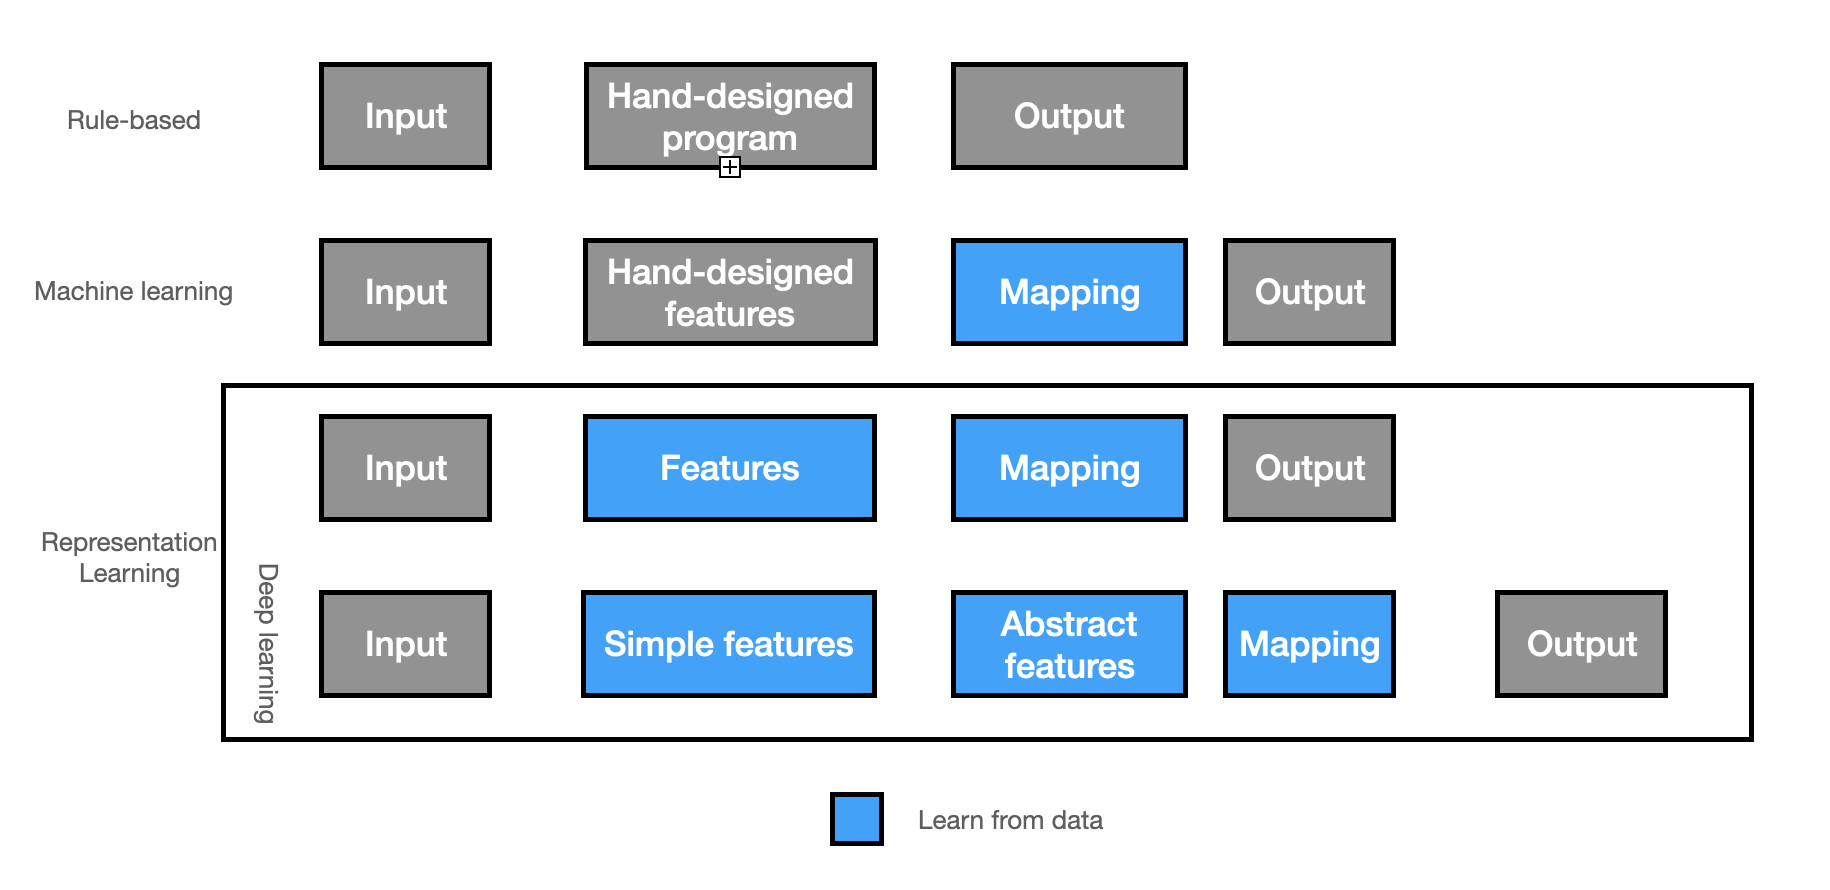
\includegraphics[width=\textwidth]{evolution-of-deep-learning.png}
  \caption{Evolution of deep learning}
  \label{fig:evolution-of-deep-learning}
\end{figure}

\chapter{Machine Learning Basics}
Machine learning is essentially a form of applied statistics with increased emphasis on the use of computers to statistically estimate complicated functions and a decreased emphasis on proving confidence intervals around these functions.


\section{Learning Algorithms}

A machine learning algorithm is an algorithm that is able to learn from data.
But what do we mean by learning?
Mitchell provides a succinct definition:
``A computer program is said to learn from experience $E$ with respect to some class of tasks $T$ and performance measure $P$, if its performance at tasks in $T$, as measured by $P$, improves with experience $E$''
Now, how does the learn happen?
The model or algorithm learns by adjusting the parameters contained in it.


\section{Capacity, Overfitting and Underfitting}

The central challenge in machine learning is that out algorithm must perform well on \itwords{new, previously} -- not just on which our model was trained.
The ability to perform on previously unobserved inputs is called \keywords{generalization}.

Typically, when training a machine learning model, we have access to a training set;
we can compute some error measure on the training set, called the \keywords{training error};
and we reduce this training error.
We simply call this an optimization problem.
What separate machine learning from optimization is that we want the \keywords{generalization error}, also called the \keywords{test error} to be low as well.
The generalization error is defined as the expected value of the error on a new input.



How can we affect performance on the test set when we get to observe only the training set? 
The field of \keywords{statistical learning theory} provides some answers. 
If the training and the test set are collected arbitrarily, there is indeed little we can do.
If we are allowed to make some \keywords{assumptions} about how the training and test set are collected, then we can make some progress.

The training and test data are generated by a probability distribution over datasets called the \keywords{data-generating process}.
We typically make a set of assumptions known as the \keywords{i.i.d. assumptions}.
These assumptions are that the examples in each dataset are independent from each other, and that the training set and test set are identically distributed, drawn from the same probability distributed as each other.
This assumption enables us to descirbe the data-generating process with a probability distribution over a single example.
The same distribution is then used to generate every train example and every test example.
We call that shared underlying distribution the \keywords{data-generating distribution}, denoted $p_{data}$.
This probability framework and the i.i.d. assumptions enables us to mathematically study the relationship between training error and test error.


One connection between training error and test error is that expected training error of a randomly selected model is equal to the expected test error of that model.
When we use a machine learning algorithm, we sample the training set, the use it to choose the parameters to reduce training set error, the sample the test set.
Under this process, the expected test error is greater than or equal to the expected value of training error.
The factors determining how well a machine learning algorithm will perform are its ability to
\begin{enumerate}
\item Make the training error small.
\item Make the gap between training and test error small.
\end{enumerate}
These two factors correspond to the two central challenges: \keywords{underfitting} and \keywords{overfitting}.
Underfitting occurs when the model is not able to obtain a sufficient low error value on the training set.
Overfitting occurs when the gap between the training error and test error is too large.

We can control whether a model is more likely to overfit or underfit by altering its \keywords{capacity}.
Informally, a model's capacity is its ability to fit a wide variety of functions.


One way to control the capacity of a learning algorithm is by choosing its hypothesis space, the set of functions that the learning algorithm is allowed to selected as being the solution.
Capacity is not determined only by the choice of model.
The model specifies which family of functions the learning algorithm can choose from.
This is called the \keywords{representation capacity} of the model.
In many cases, finding the best function within this family is a difficult optimization problem.
In practice, the learning algorithm does not actually find the best function, but merely one that sinificantly reduces the training error.
This additional limitations, such as the inperfection of the optimization algorithm, mean that the learning algorithm's \keywords{effective capacity} may be less than the representational capacity of the model family.

\begin{tcolorbox}
  Machine learning algorithm will generally perform best when their capacity is appropriate for the true complexity of the task and the amount of training data.
\end{tcolorbox}



The ideal model is an oracle that simply knows the true probability distribution that generate the data.
Even such a model will still incur some error on many problems, because there may still be some noise in the distribution.
In the case of supervised learning, the mapping from $\bm{x}$ to $y$ may be inherently stocastic, or $y$ may be a deterministic function that involves other variables besides those included in $\bm{x}$.
The error incurred by an oracle making predictions from the true distribution $p(\bm{x},y)$ is called the \keywords{Bayes error}.


\subsection{The No Free Lunch Theorem}

Learning theory claims that a machine learning algorithm can generalize well from a finite training set of examples.
However, to logically infer a rule describing every memeber of a set, one must have information about every member of that set.

In part, machine learning avoids this problem by offering only probabilistic rules, rather than the entirely certain rules used in purely logical reasoning.
Machine learning promises to find rules that are \itwords{probably} correct about \itwords{most} memebers of the set they can concern.


Unfortunately, even this does not resovle the entire problem.
The \keywords{no free lunch theorem} for machine learning states that, averaged over all possible data-generating distribution, every classification algorithm has the same error when classicifying previously unobserved points.
In other words, in some sense, no machine learning algorithm is universally any better than any other.

Fortunately, these results holds only when we average over \itwords{all} possible data-generating distribution.
If we make assumptions about the kinds of probability distributions we encounter in real-world application, then we can design learning algorithms that perform well on these distributions.


This means that the goal of machine learning research is not to seek a universal learning algorithm or the absolute best learning algorithm.
Instead, our goal is to understand what kinds of distributions are relevant to the ``real world'' that an AI agent experiences, and what kinds of machine learning algorithm perform well on data drawn from the kinds of data-generating distributions we care about.


\subsection{Regularization}

The no free lunch theorem implies that we must design our machine learning algorithms to perform well on a specific task.
We do so by building a set of preferences into the learning algorithm.

The behavior of our algorithm is strongly affacted not just by how large we make the set of functions allowed in its hypothesis space, but by the specific identity of those functions.
For example, liner regression would not perform well if we tried to use it to predict $\sin(x)$ from $x$.
We can thus control the performance of our algorithm by choosing what kind of functions we allow them to draw solutions from, as well as by controlling the amount of these functions.

Generally, we can regularize a model that learns a function $f(\bm{x};\theta)$ by adding a penalty called a \keywords{regularizer} to the cost function.
In the case of weight decay, the relularizer is $\Omega(w) = w^\top w$.

Expressing preferences for one function over anohter is a more general way of controlling a model's capacity.

\begin{tcolorbox}
  Regularization is any modification we make to a learnining algorithm that is intended to reduce its generalization error but not its training error.
\end{tcolorbox}


The no free lunch theorem has made it clear that there is no best machine learning algorithm, and in particular, no best form of regularization.
Instead we must choose a form of regularization that is well suited to the particular task we want to solve.
The philosophy of deep learning is that a wide range of tasks may all be solved effectively using very general-purpose forms of regularization.

\section{Hyperparameters and validation sets}

Most machine learning algorithms have hyperparameters, setting that we can use to control the algorithm's behavior.
The values of hyperparameters are not adapted by the learning algorithm itself.


Sometimes a setting is chosen to be a hyperparameter that the learning algorithm does not learn because the setting is difficult to optimize.
Most frequently, the setting must be hyperparameter because it is not appropriate to learn that hyperparameter on the training set.
This applies ot all hyperparameters that control model capacity.
If learned on the trainning set, sunch hyperparameters would always choose the maximum possible capacity, resulting in overfitting.


To solve this problem, we need a \keywords{validation set} of examples that the training algorithm does not observe.
It is important that the test examples are not used in any way to make choice about the model, including hyperparameters.
Therefore, we always construct the validation set from the training data.
Specifically, we split the training data into tow disjoint subsets.
The subset of data used to learn the parameters is still typically called the training set.
The subset of data used to guide the selection of hyperparameters is called the validation set.
Typically, one uses about 80 percent of the training data for training and 20 percent for validation.

\section{Estimators, bias and variance}

Foundational concepts such as parameter estimation, bias and variance are useful to formally characterize notions of generalization, underfitting and overfitting.

\subsection{Point estimation}
Point estimation is the attempt to provide the single ``best'' prediction of some quantity of interest.
To distinguish estimators of parameters from their true value, our convention will be to denote a point estimate of a parameter $\bm{\theta}$ by $\hat{\bm{\theta}}$.

Let $\{\bm{x}^{(1)},\dots,\bm{x}^{(m)}\}$ be a set of $m$ independent and identically distributed (i.i.d.) data points.
A \keywords{point estimator} or \keywords{statistic} is any function of the data:
\begin{equation}
  \hat{\bm{\theta}} = g(\bm{x}^{(1)},\dots,\bm{x}^{(m)}).
\end{equation}
While almost any function thus qualifies as an estimator, a good estimator is a function whose output is close to the true underlying $\bm{\theta}$ that generated the training data.

\subsection{Bias}

The bias of an estimator is defined as
\begin{equation}
  \mathrm{bias}(\hat{\bm{\theta}}_m) = \mathbb{E}(\hat{\bm{\theta}}_m) - \bm{\theta},
\end{equation}
where the expectation is over the data (seen as samples from a random variable) and $\bm{\theta}$ is the true underlying value of $\bm{\theta}$ used to define the data-generating distribution.
An estimator $\hat{\bm{\theta}}$ is said to be \keywords{unbiased} if $\mathrm{bias}(\hat{\bm{\theta}}_m)=0$.
An estimator  $\hat{\bm{\theta}}_m$ is said to be \keywords{asymptotically unbiased} if $\lim_{m\rightarrow \infty}\mathrm{bias}(\hat{\bm{\theta}}_m) = 0$.

\subsection{Variance and standard error}

The variance of an estimator is simply the variance
\begin{equation}
  \mathrm{Var}(\hat{\bm{\theta}})
\end{equation}
where the random variable is the training set.
Alternately, the square root of the variance is called the \keywords{standard error}, denoted $\mathrm{SE}(\hat{\bm{\theta}})$.

The variance, or the standard error, of an estimator provides a measure of how we would expect the estimate we compute from data to vary as we independently resample the dataset from the underlying data-generating process.


\begin{tcolorbox}
  When we compute any statistic using a finite number of samples, our estimate of the true underlying parameter is uncertain.
\end{tcolorbox}


\subsection{Consistency}

We usually wish that, as the number of data points $m$ in our dataset increase, our point estimates converge to the true value of the corresponding parameters.
More formally, we would like that
\begin{equation}
  \label{eq:consistency}
  \mathrm{plim}_{m\rightarrow \infty}\hat{\bm{\theta}}_m = \bm{\theta}.
\end{equation}

The symbol plim indicates convergence in probability, meaning that for any $\epsilon > 0$, $P(|\hat{\bm{\theta}}_m - \bm{\theta}| > \epsilon) \rightarrow 0$ as $m \rightarrow \infty$.
The condition described by equation \ref{eq:consistency} is known as \keywords{consistency}.


\section{Maximum likelihood estimation (*)} 

Rather than guessing that some function might make a good estimator and then analyzing its bias and variance, we would like to have some priciple from which we can derive specific functions that are good estimators for different models.

The most common such principle is the maximum likelihood estimation.


Consider a set of $m$ examples $\mathbb{X} = \{\bm{x}^{(1)},\dots, \bm{x}^{(m)}\}$ drawn independently from the true but unknown data-generating distribution $p_{data}(\mathbf{x})$.

Let $p_{model}(\mathbf{x};\theta)$ be a parametric family of probability distributions over the same space indexed by $\theta$.

The maximum likelihood estimator for $\theta$ is then defined as:
\begin{equation}
  \label{eq:maximum-likelihood}
  \bm{\theta}_{\mathrm{ML}} = \mathop{\arg\max}_{\bm{\theta}} p_{\mathrm{model}}(\mathbb{X};\bm{\theta}) =  {\arg\max}_{\bm{\theta}} \prod_{i=1}^m p_{\mathrm{model}}(x^{(i)};\bm{\theta}) 
\end{equation}

To get a convenient but equivalent optimization problem:
\begin{equation}
  \bm{\theta}_{\mathrm{ML}} = \mathop{\arg\max}_{\bm{\theta}}  \sum_{i=1}^m  \log p_{\mathrm{model}}(x^{(i)};\bm{\theta})
\end{equation}

Because the arg max does not change when we rescale the cost function, we can divide by $m$ to obtain a version of the criterion that is expressed as expectation with respect to the empirical distribution $\hat{p}_{data}$ defined by the training data:
\begin{equation}
  \bm{\theta}_{\mathrm{ML}} = \mathop{\arg\max}_{\bm{\theta}}  \mathbb{E}_{x\sim \hat{p}_{data}}  \log p_{\mathrm{model}}(x;\bm{\theta})
\end{equation}


One way to interpret maximum likelihood estimation is to view it as minimizing the dissimilarity between the empirical distribution $\hat{p}_{data}$, defined by the training set and the model distribution, with the degree of dissimilarity between the two measured by the KL divergence.
The KL divergence is given by:
\begin{equation}
  \label{eq:kl-divergence}
  D_{KL}(\hat{p}_{data}||p_{data}) = \mathbb{E}_{\mathrm{x}\sim \hat{p}_{data}} [\log \hat{p}_{data}(\bm{x}) - \log p_{model}(\bm{x})]
\end{equation}

\subsection{Properties of maximum likelihood}

The main appeal of the maximum likelihood estimator is that it can be shown to be the best estimator asymptotically, as the number of examples $m \rightarrow \infty$, in terms of its rate of convergence as $m$ increases.

Under appropriate conditions, the maximum likelihood estimator has the property of consistency.
These conditions are as follows:
\begin{itemize}
\item The true distribution $p_{data}$ must lie within the model family $p_{model}(\cdot;\theta)$.
\item The true distribution $p_{data}$ must correspond to exactly one value of $\theta$.
\end{itemize}



\section{Bayesian statistics}

In frequentist perspective, the true parameter value $\theta$ is fixed but unknown, while the point estimator $\hat{\theta}$ is a random variable on account of it being a function of the dataset.
The Bayesian perspective on statistic is quite different.
The Bayesian uses probability to reflect degrees of certainty in states of knowledge.
The dataset is directly observed and so is not random.
On the other hand, the true parameter $\theta$ is unknown or uncertain and thus is represented as a random variable.



Before observing the data, we represent out \keyword{knowledge} of $\theta$ using the \keyword{prior probability distribution}, $p(\theta)$.
Generally, the machine learning practitioner selects a prior distribution that is quite broad (i.e. with high entropy) to reflect a high degree of uncertainty in the value of $\theta$ before observing any data.
Now consider that we have a set of data samples $\{x^{(1)}, \cdots,x^{(m)}\}$.
We can recover the effect of data on our belief about $\theta$ by combining the data likelihood $p(x^{(1)},\cdots,x^{(m)}|\theta)$ with the prior via Bayes' rule:
\begin{equation}
  p(\theta|x^{(1)},\cdots,x^{(m)}) = \frac{p(x^{(1)},\cdots,x^{(m)}|\theta)p(\theta)}{p(x^{(1)},\cdots,x^{(m)})}
\end{equation}







\section{Stochastic Gradient Descent}

Nearly all of deep learning is powered by one very important algorithm: \keyword{stochastic gradient descent} (SGD).
A recurring problem in machine learning is that large training sets are neccessary for good generalization, but large training sets are also more computationally expensive.


The cost function used by a machining learning algorithm often decomposes as a sum over training examples of some per-example loss function.
For example, the negative conditional log-likelihood of the training data can be written as
\begin{equation}
  J(\bm{\theta}) = \mathbb{E}_{\mathrm{x},y \sim \hat{p}_{data}} L(\bm{x},y,\bm{\theta}) = \frac{1}{m}\sum_{i=1}^m L(\bm{x}^{(i)},y^{(i)},\bm{\theta}),
\end{equation}
where L is the per-example loss $L(\bm{x},y,\bm{\theta}) = -\log p(y|\bm{x};\bm{\theta})$.

For these additive cost function, gradient requires computing
\begin{equation}
  \nabla_{\bm{\theta}} J(\bm{\theta}) = \frac{1}{m}\sum_{i=1}^m L(\bm{x}^{(i)},y^{(i)},\bm{\theta}).
\end{equation}
The computational cost of this operation is $O(m)$.
As the training set size grows to billions of examples, the time to take a single gradient step becomes prohibitively long.

The insight of SGD is that the gradient is an expectation.
The expectation may be approximately estimated using a small set of samples.
Specifically, on each step of the algorithm, we can sample a \keyword{minibatch} of examples $\mathbb{B}=\{\bm{x}^{(1)},\cdots,\bm{x}^{(m)}\}$ drawn uniformly from the training set.
The minibatch size $m'$ is typically chosen to be a relatively small number of examples, ranging from one to a few hundred.

The estimator of the gradient is formed as
\begin{equation}
  \bm{g} = \frac{1}{m'} \nabla_{\bm{\theta}} \sum_{i=1}^{m'} L(\bm{x}^{(i)},y^{(i)},\bm{\theta})
\end{equation}
using examples from the minibatch $\mathbb{B}$.
The stocastic gradient descent algorithm then follows the estimated gradient donwhill:
\begin{equation}
  \bm{\theta} \leftarrow \bm{\theta} - \epsilon \bm{g},
\end{equation}
where $\epsilon$ is the learning rate.

\section{Building a machine learning algorithm}

Nearly all deep learning algorithms can be described as particular instances of a fairly simple recipe:
\begin{itemize}
\item a specification of a dataset
\item a cost function
\item an optimization procedure
\item a model
\end{itemize}



\section{Challenges Motivating Deep Learning}

The development of deep learning was motivated in part by the failure of traditional algorithms to generalize well on AI tasks, such as recognizing speech or recognizing objects.

\subsection{The Curse of dimensionality}

Many machine learning problems become exceedingly difficult when the number of dimenions in the data is high.
This phonomenon is known as the \keyword{curse of dimensionality}.
One challenge posed by the curse of dimensionality is a statistical challenge.
A statistical challenge arises becuase the number of possible configurations of $x$ is much large than the number of training examples.


\subsection{Local constancy and smoothness regularization}

To generalize well, machine learning algorithms need to be guided by prior beliefs about what kind of function they should learn.
Among the most widely used implicit ``priors'' is the \keyword{smoothness prior}, or local constancy prior.
This prior states that the function we learn should not change very much within a small region.

There are many different ways to implicitly or explicitly express a prior belief that the learned function should be smooth or locally constant.
All these different methods are designed to encourage the learning process to learn a function $f^{*}$ that satisfies the condition
\begin{equation}
  f^{*}(\bm{x}) \approx f^{*}(\bm{x} + \epsilon)
\end{equation}

\section{Manifold Learning}

An important concept underlying many ideas in machine learning is that of a manifold.
A \keyword{manifold} is a connected region.
Mathematically, it is a set of points associated with a neighborhood around each point.
The concept of a neighborhood surrounding each point implies the existence of transformations that can be applied to move on the manifold from one position to a neighboring one.


Many machine learning problems seem hopeless if we expect the machine learning algorithm to learn function with interesting variations across all of $\mathbb{R}^n$.
\keyword{Manifold learning} algorithms surmount this obstacle by assuming
the most of $\mathbb{R}^n$ consists of invalid inputs,and that
interesting inputs occurs only along a collection of manifolds contaning a small subset of points,
with interesting variations in the output of the learned function occuring only along directions that lie on the manifold,
or with interesting variations happening only when we move from one manifold to another.


The assumption that the data lies along a low-dimensional manifold may not always be correct or useful.
We argue that in the context of AI tasks, such as those that involve processing images, sounds, or text,
the manifold assumptions is at least approximately correct.

The evidence in favor of this assumptions consists of tow categories of observations:
\begin{enumerate}
\item The probability distribution over images, text strings, and sounds that occur in real life is highly concentrated.
\item We can imagine such neighborhoods and transformations, at least informally.
\end{enumerate}




\chapter{Deep Feedforward Networks}

\keyword{Deep feedforward networks}, also called \keyword{feedforward neural networks}, or \keyword{multilayer perceptions} (MLPs), are the quintessential deep learning models.
The goal of a feedforward network is to approximate some function $f^{*}$.
A feedforward network defines a mapping $\bm{y} = f(\bm{x};\bm{\theta})$ and learns the value of the parameter $\bm{\theta}$ that result in the best function approximation.


These models are called \keyword{feedforward} because information flows through the function being evaluated from $\bm{x}$, through the intermediate computations used to define $f$, and finally to the output $\bm{y}$.
Feedforward neural network are called \keyword{networks} becuase they are typically represented by composing together many different functions.


\section{Gradient-Based Learning}

The nonlinearity of a neural network causes most intersting loss functions to become nonconvex.
This means that neural networks are usually trained by using iterative, gradient-based optimizer that merely drive the cost function to a very low value.
Convex optimization converges starting from any initial parameters.
Stochastic gradient descent applied to nonconvex loss functions has no such convergence guarantee and is sensitive to the values of the initial parameters.




\chapter{Regularization for Deep Learning}

A central problem in machine learning is how to make an algorithm that will perform well not just on the training data, but also on new inputs.
Many strateries used in machine learning are explicitly designed to reduce the test error, possibly at the expense of increased training error.
These strateries are known collectively as \keyword{regularization}.


In practice, an overly complex model family does not necessarily include the target function or the true data generating process, or even a close approximation of either.
We almost never have access to the true data generating process so we can never know for sure if the model family being estimated includes the generating process or not. 
However, most applications of deep learning algorithms are to domains where the true data generating process is almost certainly outside the model family. 
Deep learning algorithms are typically applied to extremely complicated domains such as images, audio sequences and text, for which the true generation process essentially involves simulating the entire universe. 
To some extent, we are always trying to fit a square peg (the data generating process) into a round hole (our model family).


What this means is that controlling the complexity of the model is not a simple matter of finding the model of the right size, with the right number of parameters.
Instead, we might find -- and indeed in practical deep learning scenarios, we almost always do find -- that the best fitting model is a larger model that has been regularized appropriately.


\section{Parameter Norm Penalties}

Many regularization approaches are based on limiting the capacity of models by adding a parameter norm penalty $\Omega(\bm{\theta})$ to the objective function $J$.
\begin{equation}
  \label{eq:norm-penalties}
  \tilde{J}(\bm{\theta;X,y}) = J(\bm{\theta,X,y}) + \alpha \Omega(\bm{\theta})
\end{equation}



\subsection{$L^2$ Parameter Regularization}

The $L^2$ parameter norm penalty commonly known as \keyword{weight decay}.
This regularization strategy derives the weights closer to the original by adding a regularization term $\Omega(\bm{\theta}) = \frac{1}{2} ||\bm{w}||_2^2$ to the objective function.


\subsection{$L^1$ Regularization}

$L^1$ regularization on the model parameter $\bm{w}$ is defined as
\begin{equation}
  \label{eq:l1}
  \Omega(\bm{\theta}) = ||\bm{w}||_1 = \sum_i |w_i|.
\end{equation}


\section{Dataset Augmentation}

The best way to make a machine learning model generalize better is to train it on more data.
Of course, in practice, the amount of data we have is limited.
One way to get around this problem is to create fake data and add it to the training set.


Dataset augmentation has been a particular effective technique for a specific classification problem: object recognition.

\section{Noise Robustness}

For some models, the addition of noise with infinitesimal variance at the input of hte model is equivalent to imposing a penalty on the norm of the weights.
In the general case, it is important to remember that noise injection can be much more powerful than simply shrinking the parameters, especially when the noise is added to the hidden units.



\section{Semi-Supervised Learning}

In the paradigm of semi-supervised learning, both unlabeled examples from $P(\mathrm{x})$ and labeled examples from $P(\mathrm{x,y})$ are used to estimate $P(\mathrm{y|x})$ or predict $\mathrm{y}$ from $\mathrm{x}$.


In the context of deep learning, semi-supervised learning usually refers to learning a representation $\bm{h} = f(\bm{x})$. The goal is to learn a representation so that examples from the same class have similar representations.



\section{Multitask Learning}


Multitask learning is a way to improve generalization by pooling the examples (which can be seen as soft constaints imposed on the parameters) arising out of several tasks.
In the same way that additional tranining examples put more pressure on the parameters of the model toward values that generalize well, when part of a model is shared across tasks, that part of the model is more constrained toward good values (assuming the sharing is justified), often yielding better generalization.



\section{Early Stopping}

Early stopping is used to avoid overfit.

The algorithm terminates when no parameters have improved over the best recorded validation error for some pre-specified number of iterations.
This strategy is known as \keyword{early stopping}.
It is probably the most commonly used form of regularization in deep learning.


Early stopping is a unobtrusive form of regularization, in that it requires almost no change in the underlying training procedure, the objective function, or the set of allowable parameter values.
Early stopping requires a validation set, which means some traning data is not fed to the model.



\section{Parameter Tying and Parameter Sharing}

Sometimes we want to express our prior knowledge about suitable values of the model parameters.
Sometimes we might not know precisely what values the parameters should take, but we know, from knowledge of the domain and model archtecture, that there should be some dependencies between the model parameters.

A common type of dependency that we foten want to express is that certain parameters should be close to one another.
For example:
We have model A with parameters $\bm{w}^{(A)}$ and model B with parameters $\bm{w}^{(B)}$.
We believe the model parameters should be close to each other: $\forall i w_i^{(A)}$ should be close to $w_i^{(B)}$.
We can use a parameter norm penalty of the form $\Omega(\bm{w}^{(A)},\bm{w}^{(B)} = || \bm{w}^{(A)} - \bm{w}^{(B)} ||_2^2$.
Here we use an $L^2$ penalty, but other choices are also possible.
This is called \keyword{parameter typing}.


While a parameter norm penalty is onw way to regularize parameters to be close to one another, the more popular way is to use constraints:
\textit{to force stes of parameters to be equal}.
This method of regularization is often referred to as \keyword{parameters sharing}, because we interpret the various models or model components as sharing a unique set of parameters.


\section{Sparse Representations}


Weightdecay acts by placing a penalty directly on the model parameter.
Another strategy is to place a penalty on the activation of the units in a neural network, encouraging their activation to be sparse.
This indirectly imposes a complicated penalty on the model parameters.


\section{Bagging and Other Emsemble Methods}

Bagging (short for bootstrap aggregating) is a technique for reducing generalization erry by combining several models.
The idea is to  train several different models separately, then have all the models vote on the output for test examples.
This is a exampe of a general strategy in machine learning called model averaging.
Techniques employing this strategy are known as \keyword{ensemble methods}.

The reason that model averaging works is that different models will usually not make all the same error on the test set.


\section{Adversarial Training}

Szegedy et al. (2014b) found that even neural network that perform at human level accuracy have a nearly 100 percent error rate on examples that are intentionally constructed by using an optimization procedure to search for an input $x^{'}$ near a data point $x$ such that the model output is very different at $x^{'}$.
In many cases, $x^{'}$ can be so similar to $x$ that a human observe cannot tell the difference between the original example and the \keyword{adversarial example}, but the network can make highly different predictions.


We can reduce the error rate on the original i.i.d. test set via adversarial training -- training on adversarially perturbed examples from the training set.

\chapter{Optimization for Training Deep Models}



\chapter{Convolutional Networks}

\keyword{Convolutional networks}, also known as \keyword{convolutional neural networks} or CNNs, are specialized kind of neural network for processing data that has a known \keyword{grid-like} topology.
Convolution is a specialized kind of linear operation.
Convolutional networks are simply neural networks that use convolution in place of general matrix multiplication in at least one of their layers.


\section{The Convolution Operation}

\begin{equation}
  \label{eq:convolution}
  s(t) = \int x(a)w(t-a)da.
\end{equation}
This operation is called \keyword{convolution}.
The convolution operation is typically denoted with an asterisk:
\begin{equation}
  s(t) = (x*w)(t).
\end{equation}

In convolutional network terminology, the first argument (in this example, the function $x$) to the convolution is often referred to as the \keyword{input}, and the second argument (int this example, the function $w$) as the \keyword{kernel}.
The output is sometimes referred to as the \keyword{feature map}.

If we assume that $x$ and $w$ are defined only on integer $t$, we can define the discrete convolution:
\begin{equation}
  \label{eq:discrete-convolution}
  s(t) = (x*w)(t) = \sum_{a=-\infty}^{\infty} x(a)w(t-a).
\end{equation}


We often use convolutions over more than one axis at a time.
For example, if we use a two-dimensinal image $I$ as our input, we probably also want to use a two-dimensional kernel $K$:
\begin{equation}
  S(i,j) = (I*K)(i,j) = \sum_m\sum_n I(m,n)K(i-m,j-n).
\end{equation}


Convolution is commulative, meaning we can equivalently write
\begin{equation}
  S(i,j) = (K*I)(i,j) = \sum_m\sum_n I(i-m,j-n)K(m,n).
\end{equation}

Usually the latter formula is more stratghtforward to implement in a machine learning library, because there is less variation in the range of valid values of $m$ and $n$.


The commulative property of convolution arises becuase we have fipped the kernel relative to the input, in the sense that as $m$ increase, the index into the input increase, but the index into the kernel decrease.
The only reason to flip the kernel is to obtain the commulative property.
While the commulative property is useful for writting proofs, it is not usually an important property of a neural network implementation.
Instead, many neural network libraries implement a related function called the \keyword{cross-correlation}, which is the same as convolution but without flippling the kernel:
\begin{equation}
  S(i,j) = (I*K)(i,j) = \sum_m\sum_nI(i+m,j+n)K(m,n).
\end{equation}
Many machine learning libraries implement cross-correlation but call it convolution.


\section{Motivation}

Convolution leverages three important ideas:
\begin{itemize}
\item sparse interaction.
\item parameter sharing.
\item equivariant representations.
\end{itemize}

\subsection{Sparse interaction}

Tradition neural network layers use matrix multiplication by a matrix of parameters with a separate parameter describing the interaction between each input unit and each output unit.
This means that every output unit interacts with every input unit.
Convolutional networks typically have sparse interactions.
This is accomplished by making the kernel smaller than the input.


\subsection{Parameter sharing}

Parameter sharing refers to use the same parameter for more than one function in a model.
In a traditional nerual net, each element of the weight matrix is used exactly once when computing the output of a layer.
It is multiplied by one element of the input and then never revisited.
In a convolutional neural net. each member of the kernel is used at every postion of the input.
The parameter sharing used by the convolution operation means that rather than learning a separate set of parameters for every location, we learn only one set.

\subsection{Equivariant representations}

In the case of convolution, the particular form of a parameter sharing causes the layer to have a property called \keyword{equivariance} to translation.
To say a function is equivariant means that if the input changes, the output changes in the same way.
Specifically, a function $f(x)$ is equivariant to a function $g$ if $f(g(x)) = g(f(x))$.
In the case of convolution, if we let $g$ be any function that translate the input, that is, shifts it, then the convolution function is equivalent to $g$.

For images, convolution creates a 2-D map of where certain features appear in the input.
If we move the object in the input, its representations will move the same amount in the output.
This is useful for when we know that some function of a small number of neighboring pixels is useful when applied to multiple input location.
For example, when processing images, it is useful to detect edges in the first layer of a convolutional network,
The same edges appear more or less everywhere in the image, so it is practical to share parameters across the intire image.

Convolution is not naturally equivalent to some other transformation, such as changes in the scale or ratation of a image.




\section{ Pooling}

A typical layer of a convolutional network consists of three stages:
\begin{enumerate}
\item convolution stage: affine transform
\item detector stage: nonlinearty
\item pooling stage
\end{enumerate}


In the first stage, the layer performs several convolutions in parallel to produce a set of linear activations.
In the second stage, each linear activations is run through a nonlinear activation function, such as the rectified linear activation function.
In the third stage, we use a pooling function to modify the output of the layer further.


A pooling function replaces the output of the net at a certain location with a summary statistic of the nearby outputs.
For example, the max pooling oeration reports the maximum otuput within a rectangular neighborhood.
Other popular pooling functions include the average of a rectangular neighborhood,
the $L^2$ norm of a rectangular neighborhood, or a weighted average based on the distance from the central pixel.


In all cases, pooling helps to make the representation approximately invariant to small translations of the input.
Invariant to translation means that if we translate the input by a small amount, the values of most of the pooled outputs do not change.
Invariance to local translation can be a useful property if we care about whether some feature is present than exactly where it is.
For example, when determining whether an image contains a face, we need not know the location of the eyes with pixel-perfect accuracy,
we just need to know that there is an eye on the left side of the face and an eye on the right side of the face.
In ohter example, it is more important to perserve the location of a feature.
For example, if we want to find a corner defined by two edges meeting at a specified orientation,
we need to perserve the location of the edge well enough to test whether they meet.


The use of pooling can be viewed as adding a infinitly strong prior that the function the layer learns must be invariant to small translations.
When this assumption is correct, it can greatly improve the statistical efficiency of the network.


\section{Convolution and Pooling as an Infinitely Strong Prior}

A probability distribution over the parameters of a model encodes our beliefs about what models are reasonable, before we see any data.

Prior can be considered weak or strong depending on how concertrated the probability density in the prior is.
A weak prior is a prior distribution with high entropy.
A strong prior is a prior distribution with low entropy.
An infinitely strong prior places zero probability on some parameters and says that these parameter values are completely forbidden,
regardless of how much support the data give to these values.


We can imagine a convolutional net as being similar to a fully connected net, but with an infinitely strong prior over its weights.
This infinitely strong prior says that the weights for one hidden unit must be identical to the weights of its neighbor, but shifted in space.
The prior also says that the weights must be zero, except for in the small, spatially contiguous receptive field assigned to that hidden unit.
Overall, we can think of the use of convolution as introducing an infinitely strong prior probability distribution over the parameters of a layer.
This prior says that the function the layer should learn contains only local interactions and is equivariant to translation.
Likewise, the use of pooling is an infinitely strong prior that each unit should be invariant to small translations.




\section{Structured Outputs}

Convolutional networks can be used to output a high-dimensional, structured object, rather than just predicting a class label for a classification task or a real value for a regression task.
Typically this object is just a tensor, emitted by a standard convolutional layer.
For example, the model might emit a tensor $S$, where $S_{i,j,k}$ is the probability that pixel $(j,k)$ of the input to the network belongs to class i.
This allows the model to label every pixel in an image and draw precise masks that follow the outlines of individual objects.
This the basis of the segmentation model.



In the kinds of architectures typically used for classification of a single object in an image, the greatest reduction in the spatial dimensions of the network comes from using pooling layers with large stride.
To produce an output map of similar size as the input, one can:
\begin{itemize}
\item avoid pooling altogether
\item emit a lower-resolution grid of labels
\item use a pooling operator with unit stride
\end{itemize}




\chapter{Practical Methodology}

Successfully applying deep learning techniques requires more than a good knowledge of what algorithms exist and
the principles that explain how they work.
A good machine learning practitioner also needs to know how to choose an algorithm for a particular application and
how to monitor and respond to feedback obtained from experiments in order to improve a machine learning system.
Practitioners need to decide whether to gather more data,
increase or decrease model capacity,
add or remove regularizing features,
improve the optimization of a model,
improve approximate inference in a model,
or debug the software implementation of the model.


\begin{tcolorbox}
  \begin{itemize}
  \item a good knowledge of what algorithms exist
  \item the principles that explain how they work
  \item how to choose an algorithm for a particular application
  \item how to monitor and respond to feedback
    \begin{itemize}
    \item whether to gather more data
    \item increase or decrease model capacity
    \item add or remove regularizing features
    \item improve the optimization 
    \item improve approximate inference
    \item debug the software
    \end{itemize}
  \end{itemize}
\end{tcolorbox}


Some practical process:
\begin{enumerate}
\item Determine your goal -- what error metric to use, and your target value for this error metric.
  These goals and error metrics should be driven by the problem that the application is intended to solve.
\item Establish a working end-to-end pipeline as soon as possible, including the estimation of the appropriate performance metrics.
\item Instrument the system well to determine bottlenecks in performance.
  Diagnose which components are performing worse than expected and whether poor performance is due to overfitting, underfitting, or a defect in the data or software.
\item Repeatedly make incremental changes such as gathering new data, adjusting hyperparameters, or changing algorithms, based on specific findings from your instrumentation.
\end{enumerate}



\part{Computer Vision Practice}

\chapter{Classification}



\chapter{Object Detection}



\chapter{Segmentation}



\chapter{Generative Model}




% \listoftables
% \listoffigures


\chapter{Gloassary}


\section{Example and features}
Machine learning tasks are usally described in terms of how the machine learning system should process an \keywords{example}.
Each piece of information included in the representation of the data is known as a \keywords{feature}.

For example,
\begin{verbatim}
Pclass,Name,Sex,Age,SibSp,Parch,Ticket,Fare,Cabin,Embarked
3,"Braund, Mr. Owen Harris",male,22,1,0,A/5 21171,7.25,,S
1,"Cumings, Mrs. John Bradley (Florence Briggs Thayer)",female,38,1,0,PC 17599,71.2833,C85,C
3,"Heikkinen, Miss. Laina",female,26,0,0,STON/O2. 3101282,7.925,,S
\end{verbatim}

There are 3 examples:
\begin{itemize}
\item \verb|3,"Braund, Mr. Owen Harris",male,22,1,0,A/5 21171,7.25,,S|
\item \verb|1,"Cumings, Mrs. John Bradley (Florence Briggs Thayer)",female,38,1,0,PC 17599,71.2833,C85,C|
\item \verb|3,"Heikkinen, Miss. Laina",female,26,0,0,STON/O2. 3101282,7.925,,S|
\end{itemize}

There are 10 features in each example:
\begin{itemize}
\item Pclass
\item Name
\item Sex
\item Age
\item SibSp
\item Parch
\item Ticket
\item Fare
\item Cabin
\item Embarked
\end{itemize}

\section{Dataset, data points and design matrix}

A dataset is a collection of many examples.
Sometimes we call examples \keywords{data points}.
A design matrix is a matrix containing a different example in each row.

\section{Unsupervised and supervised learning algorithm}

Machine learning algorithms can be broadly categorized as \keywords{unsupervised} or \keywords{supervised} by what kind of experience they are allowed to have during the learning process.
Unsupervised learning algorithms experience a dataset containing many features, then learn useful properities of the structure of this dataset.
Supervised learning algorithms experience a dataset containing many features, but each example is also associated with a \keywords{label} or \keywords{target}.

\section{Reinforcement learning}

Reinforcement learning algorithms interact with an environment, so there is a feedback loop between the learning system and its experiences.


\section{Bayes error}

The ideal model is an oracle that simply knows the true probability distribution that generate the data.
Even such a model will still incur some error on many problems, because there may still be some noise in the distribution.
In the case of supervised learning, the mapping from $\bm{x}$ to $y$ may be inherently stocastic, or $y$ may be a deterministic function that involves other variables besides those included in $\bm{x}$.
The error incurred by an oracle making predictions from the true distribution $p(\bm{x},y)$ is called the \keywords{Bayes error}.


\section{Occam's razor}

Among competing hypotheses that explain known observations equally well, we should choose the ``simplest'' one.


\section{No free lunch theorem}

The \keywords{no free lunch theorem} for machine learning states that, averaged over all possible data-generating distribution, every classification algorithm has the same error when classicifying previously unobserved points.
In other words, in some sense, no machine learning algorithm is universally any better than any other.

\backmatter
\bibliographystyle{plainnat}
\bibliography{tex}
\end{document}
